\documentclass[a4paper, justified,marginals=raggedright]{tufte-handout}


\usepackage[utf8]{inputenc}
\usepackage{graphicx} % allow embedded images
  \setkeys{Gin}{width=\linewidth,totalheight=\textheight,keepaspectratio}
  \graphicspath{{graphics/}} % set of paths to search for images
\usepackage{amsmath}  % extended mathematics
\usepackage{amssymb}  % more math symbols
\usepackage{booktabs} % book-quality tables
\usepackage{units}    % non-stacked fractions and better unit spacing
\usepackage{multicol} % multiple column layout facilities
\usepackage{fancyvrb} % extended verbatim environments
  \fvset{fontsize=\normalsize}% default font size for fancy-verbatim environments
\usepackage{pgfplots}

\usepackage{lipsum}

% to see the margins and page width
% \geometry{showframe}

% Write packages versions in the log
% \listfiles


% Commands use to make the title page and page headers
\title{Why and how to craft a trade-of in a plant functioning model}
\author{Clément Viguier}

% Commands use through the document


% Include documents for graphical aspects
% Color
%\input{../latex_settings/colors}
% Graph settings
\pgfplotsset{compat=newest}

\pgfplotsset{plot/.style={ 
width = \textwidth,
no markers,
color = black,
line width = 1pt,
minor x tick num = 0,
minor y tick num = 0,
        xtick pos=left,
        ytick pos=left,
        tick align=outside,
        try min ticks=2,
        max space between ticks=100pt,
  axis x line*=bottom,
  axis y line*=left,
        line join=round,
    axis line style={->}, 
        enlarge x limits=true,
        every x tick/.style={color=black, thin},
        every y tick/.style={color=black, thin},
}
}


\pgfplotsset{marginplot/.style={ 
plot,
width = \marginparwidth
}
}

\pgfplotsset{fullplot/.style={ 
plot,
width = \pagewidth
}
}

\begin{document}
\maketitle
\begin{fullwidth}
\begin{abstract}
\noindent
This document describes why and how a trade-of has be designed in the model MountGrass. This trade-of has the objective to allow for different strategy based on the level of resources. The same trade-of is used in shoot and roots. Parameters effects over the phenotype determination is explored for a balanced design where area cost is the same for both organs.
\end{abstract}
\end{fullwidth}

\section{Why a trade-of}
different conditions = different phenotypes\\
could be anything, needed one. Explain WUE, nitrogen and others. Try to keep independences between strategy axis to keep it simple.\\
Need for plastic driver. Explain the role of plasticity.

\section{How to craft a trade-of}

\indent The idea of trade-of suggest that you cannot invest in all strategies at the same time. To be relevant, it must be associated to a range conditions favouring different strategies along this trade-of. In other word, depending on a position on a gradient, the gradient should lead different niches. This can be visualizes as Gaussian's curves (see figure \ref{fig:niches})

\begin{marginfigure}[-30mm]
\begin{tikzpicture}
\begin{axis}[marginplot,
legend style
={at={(1, 1.1)},
anchor=south east,
draw = none},
samples = 40]

\addplot[teal][domain = 0:1 ] {exp(-(x - 0.4)^2/0.02)};
\addplot[orange][domain = 0:1 ]{exp(-(x - 0.6)^2/0.02)};
\legend{Conditions 1, Conditions 2, Conditions 3}
\end{axis}
\end{tikzpicture}
\label{fig:niches}
\caption{Different niches corresponding to different environmental conditions.}
\end{marginfigure}

The challenge is to go beyond the Gaussian function, and craft these niches from the plant physiology and ecology. Taking as a basis the usual functions used in plant modelling and the theoretical background upon which MountGrass is built, we will try to model different niches.\\

\indent In MountGrass, the Leaf Economic spectrum (LES)\cite{Wright-2004} is explained by a differential investment between active and structural tissues (supported by analysis of Shipley\cite{Shipley}). This allocation constitutes a major strategic differentiation axis, along which plastic plants can move to optimize their fitness. To keep the approach simple, we hypothesize that such trade-off would also rule the allocation of organic matter in the below-ground compartment\cite{Reich-2014; Tjoelker-2005}. As explained above, plant can modify both the shoot:root ratio, and the relative proportion of active tissues in shoot, and in roots. The first dimension is mainly driven by a balance between availability of above-ground versus below-ground resource, while the second can be driven by other strategic aspects.\footnote{This part does not belong to this section.}\\
\subsection{Crafting a trade-of for shoot}
\indent The aim of this paragraph is explain how to set up a shared plasticity mechanism that allow different phenotypes to emerge from different estimations of climatic conditions. The general principle exposed earlier is illustrated here with the example of shoot allocation strategies in MountGrass.\\
\indent Carbon allocation is driven by a gain function that quantify daily gain of the examined phenotype. This is goes against the general principle of maximizing the overall fitness, but we hypothesize that the optimization of daily gain function participates to the optimization of overall fitness function. The daily gain function is described as follow:
\begin{equation}
sdf= qsdf
\end{equation}
It is composed by the gross gain function that determine the amount of carbon assimilated by the organ during a day, and the loss function, itself the sum of respiration and turn-over cost (loss of organic matter). The net gain function result from the difference between these two functions. In order to have an optimum for $ 0 < p_{act} < 1$, the loss function must have a greater power than the gross gain function. Since, the respiration and carbon assimilation have linear relationships with $p_{act}$, the net gain function can be rewritten as follow :
\begin{equation}
qsdf =qsd 
\end{equation} 
with $\gamma > 1$.  

\begin{marginfigure}[-60mm]
\begin{tikzpicture}
\begin{axis}[marginplot,
legend style
={at={(1, 1.1)},
anchor=south east,
draw = none},
samples = 40,
restrict y to domain=-2000:2000,
xlabel = $p_{act}$]

\addplot[teal][domain = 0:1 ] {(1/(0.022 * 1)) * (1/1 + (1/0.05 - 1)*x) };
\addplot[orange][domain = 0:1 ]{1/exp(5.5)*((1/(0.022 * 1)) * (1/1 + (1/0.05 - 1)*x))^(1.8) + 0.3*x};
%\addplot[gray][domain = 0:1] {(exp(6) * ((1/(0.022 * 1)) * (1/1 + (1/0.05 - 1)*x))^(1.2)};
\legend{$Gross~gain$, $Resp + TO~loss$}
\end{axis}
\end{tikzpicture}
\label{fig:gain_cost}
\caption{Comparison of "gain" function and "cost" function. Parameter values: $\rho_{act} = 0.05$, $\rho_{str} = 1$,  $k = 7$ and  $vol_prop = 1$. The area between the two curves is the total gain by the plant.}
\end{marginfigure}


\begin{figure}
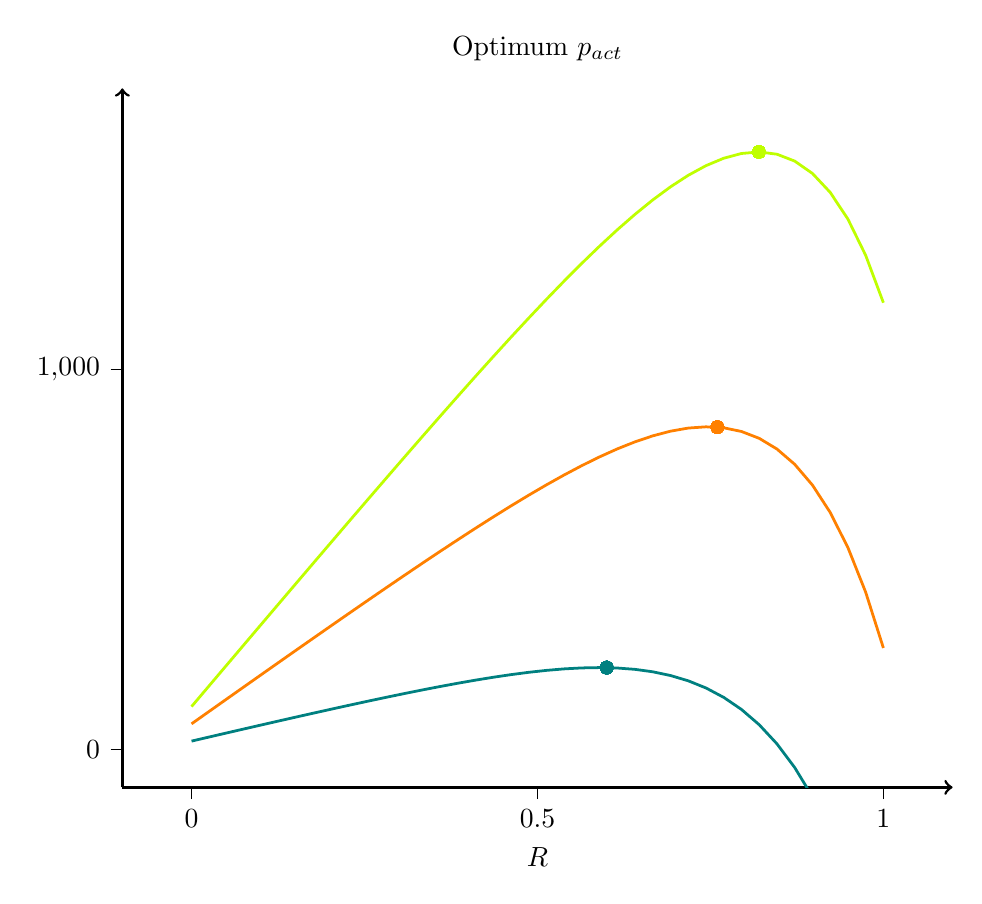
\begin{tikzpicture}
\begin{axis}[plot,
legend style
={at={(1, 0.1)},
anchor=south east,
draw = none},
samples = 40,
restrict y to domain=-2000:2000,
title = Optimum $p_{act}$,
xlabel = $R$,
ymin = -100]

% R*( g1 + g2 p_act ) − ( e(k.p_act)+ r1 .p_act )
% g1 = 1:(th*vt_s) * (1/tho_ss) = 1/0.022
% g2 = 1:(th*vt_s) * (1/rho_as - 1/tho_ss) = 1/0.022 * (1/0.05 - 1)
\addplot[teal][domain = 0:1 ] {0.5 * 1/0.022 * (1+(1/0.05 - 1)*x) - (exp(7*x) + 0.03*x)};
\addplot[orange][domain = 0:1 ] {1.5 * 1/0.022 * (1+(1/0.05 - 1)*x) - (exp(7*x) + 0.03*x)};
\addplot[lime][domain = 0:1 ] {2.5 * 1/0.022 * (1+(1/0.05 - 1)*x) - (exp(7*x) + 0.03*x)};
\addplot[teal][domain =  0.6:0.6001, only marks]{0.5 * 1/0.022 * (1+(1/0.05 - 1)*x) - (exp(7*x) + 0.03*x)};
\addplot[orange][domain =  0.76:0.76001 , only marks]{1.5 * 1/0.022 * (1+(1/0.05 - 1)*x) - (exp(7*x) + 0.03*x)};
\addplot[lime][domain =  0.82:0.82001, only marks]{2.5 * 1/0.022 * (1+(1/0.05 - 1)*x) - (exp(7*x) + 0.03*x)};
\end{axis}
\end{tikzpicture}
\label{fig:optimum}
\caption{$\blacktriangleleft$ Comparison of "gain" function and "cost" function. Parameter values: $g_{2} = $, $g_{2} = $,  $k = 7$}
\end{figure}


\begin{marginfigure}
\begin{tikzpicture}
\begin{axis}[marginplot,
legend style
={at={(1, 1.1)},
anchor=south east,
draw = none},
samples = 40,
restrict y to domain=-300:700,
xlabel = $p_{act}$,
extra x ticks={0.618},
extra x tick style={grid=major}]

\addplot[darkgray][domain = 0:1 ] {(1/(0.022 * 1)) * (1 + (1/0.05 - 1)*x) - (exp(7*x) + 0.03*x)};
\addplot[gray][domain = 0:1 ] {(1/(0.022 * 1)) * ((1/0.05 - 1)*x) - (7*exp(7*x) + 0.03)};
\legend{$Net~gain$, $f'$}
\end{axis}
\end{tikzpicture}
\label{fig:derivaives}
\caption{Net gain function and its first derivative.} Looks like there is some kind of mismatch here.
\end{marginfigure}

\subsection{How about root}
Root fol

\subsection{How do the two trade-of merge ?}
The complexity of the model is that different objectives are in line to maximize the fitness: the optimization of carbon allocation at the scale of the organ (organ efficiency), the equilibrium between the organ (whole plant balance), and other mechanisms at the plant scale (reproduction, reduction of grazing or frost risk). All these components are translated into carbon gain and losses and summed to give the net gain function. Two major components influence the balance between these components (and the resulting phenotype): the weight of species specific memory in future estimation, and the distance from optimum for each sub-function. 


\end{document}